\documentclass[10pt, aspectratio=169]{beamer}

% --- PAQUETES ---
\usepackage{lmodern}
\usepackage[spanish]{babel}
\usepackage[utf8]{inputenc}
\usepackage[T1]{fontenc}
\usepackage{amsmath, amsfonts, amsthm, amssymb}
\usepackage{mathtools}
\usepackage{subcaption}
\usepackage{xcolor}
\usepackage{tikz}
\usetikzlibrary{arrows.meta, positioning, shapes, calc, backgrounds}
\usepackage{booktabs}
\usepackage{colortbl}
\usepackage{caption}

% --- TEMA Y COLORES PERSONALIZADOS ---
\usetheme{Madrid}
\usecolortheme{whale}

\usefonttheme{professionalfonts}

\captionsetup{font=scriptsize}
\captionsetup{skip=1pt}
\captionsetup[subfigure]{skip=5pt}

\definecolor{NavyDark}{HTML}{0F172A}
\definecolor{SlateHeader}{HTML}{1E293B}
\definecolor{BlueAccent}{HTML}{2563EB}
\definecolor{TealAccent}{HTML}{0D9488}
\definecolor{AmberAccent}{HTML}{D97706}
\definecolor{RedAccent}{HTML}{DC2626}
\definecolor{LightBG}{HTML}{F8FAFC}

\setbeamercolor{palette primary}{bg=NavyDark, fg=white}
\setbeamercolor{palette secondary}{bg=SlateHeader, fg=white}
\setbeamercolor{palette tertiary}{bg=BlueAccent, fg=white}
\setbeamercolor{structure}{fg=BlueAccent}

\setbeamercolor{titlelike}{bg=NavyDark, fg=white}
\setbeamercolor{frametitle}{bg=NavyDark, fg=white}
\setbeamercolor{block title}{bg=SlateHeader, fg=white}
\setbeamercolor{block body}{bg=LightBG, fg=black}
\setbeamercolor{block title alerted}{bg=AmberAccent, fg=white}
\setbeamercolor{block body alerted}{bg=LightBG, fg=black}
\setbeamercolor{block title example}{bg=TealAccent, fg=white}
\setbeamercolor{block body example}{bg=LightBG, fg=black}

\setbeamertemplate{navigation symbols}{}
\setbeamertemplate{footline}[frame number]

% --- METADATOS ---
\title[Modelo Leslie-Gower Sigmoide]{Análisis Cualitativo y Bifurcación de Bautin en un Modelo Presa-Depredador de Leslie-Gower con Respuesta Funcional Sigmoidea}
\subtitle{Trabajo de Grado - Pregrado en Matemáticas}
\author[Y. D. Chilito Inga]{Yerson Danilo Chilito Inga}
\institute[Unicauca]{Universidad del Cauca \\ Facultad de Ciencias Naturales, Exactas y de la Educación \\ Departamento de Matemáticas}
\date{4 de noviembre de 2026}

\begin{document}
	
	% -----------------------------------------------------------------------------
	% PORTADA
	% -----------------------------------------------------------------------------
	\begin{frame}
		\titlepage
	\end{frame}
	
	% -----------------------------------------------------------------------------
	% ÍNDICE DE CONTENIDOS
	% -----------------------------------------------------------------------------
	\begin{frame}{Estructura de la Presentación}
		\tableofcontents
	\end{frame}
	
	% =============================================================================
	% SECCIÓN 1: FORMULACIÓN DEL MODELO
	% =============================================================================
	\section{Formulación del Modelo}
	
	\begin{frame}{Formulación Ecológica y Adimensionalización}
		Consideramos el modelo presa-depredador de Leslie-Gower con respuesta funcional de Holling tipo III (sigmoidea):
		\begin{equation*}
			\begin{cases} 
				\dfrac{dx}{dt} = \left[ r \left(1 - \dfrac{x}{K}\right) - \dfrac{q x y}{x^2 + a^2} \right] x, \\
				\dfrac{dy}{dt} = s \left(1 - \dfrac{y}{n x}\right) y,
			\end{cases}
		\end{equation*}
		definido en $\Omega = \{ (x,y) \in \mathbb{R}^2 \mid x > 0, \; y \geq 0 \}$ con parámetros $(r, a, s, K, n, q) \in \mathbb{R}^6_+$.
		
		\begin{block}{Adimensionalización y Reescalamiento Temporal}
			Aplicando $x = Ku$, $y = nKv$ y el reescalado temporal $d\tau = \frac{r}{u(u^2+A^2)} dt$, se obtiene el sistema polinomial topológicamente equivalente definido en $\tilde{\Omega} = \{ (u,v) \in \mathbb{R}^2 \mid u \geq 0, \; v \geq 0 \}$:
			\begin{equation*}
				\begin{cases} 
					\dfrac{du}{d\tau} = \big[(1-u)(u^2+A^2) - Q u v\big] u^2, \\[4pt]
					\dfrac{dv}{d\tau} = B (u-v)(u^2+A^2) v,
				\end{cases}
			\end{equation*}
			donde $A = \frac{a}{K} \in (0, 1)$, $Q = \frac{qn}{r} > 0$, $B = \frac{s}{r} > 0$.
		\end{block}
	\end{frame}
	
	% =============================================================================
	% SECCIÓN 2: REGIÓN INVARIANTE
	% =============================================================================
	\section{Región Invariante}
	
	\begin{frame}{Conjunto Compacto Positivamente Invariante}
		\begin{block}{Lema (Cuadrado Unitario Invariante)}
			El cuadrado cerrado $\Gamma = \{(u,v) \in \mathbb{R}^2 \mid 0 \le u \le 1, \; 0 \le v \le 1\}$ es una región positivamente invariante para el sistema adimensional.
		\end{block}
		
		\begin{columns}
			\begin{column}{0.55\textwidth}
				\textbf{Análisis de los Vectores de Flujo en $\partial\Gamma$:}
				\begin{itemize}
					\item \textbf{En $u = 0$:} $\dot{u} = 0$, $\dot{v} = -A^2 B v^2 \le 0$ (el eje $v$ es invariante).
					\item \textbf{En $v = 0$:} $\dot{u} = (1-u)(u^2+A^2)u^2 \geq 0$, $\dot{v} = 0$ (eje $u$ invariante).
					\item \textbf{En $u = 1$:} $\dot{u} = -Q v \le 0$, el flujo apunta hacia la izquierda.
					\item \textbf{En $v = 1$:} $\dot{v} = B(u-1)(u^2+A^2) \le 0$, el flujo apunta hacia abajo.
				\end{itemize}
				\textit{Conclusión:} Ninguna trayectoria puede abandonar $\Gamma$, garantizando el acotamiento biológico.
			\end{column}
			
			\begin{column}{0.42\textwidth}
				\centering
				\begin{figure}
					\begin{tikzpicture}[scale=3, >=Stealth]
						\fill[blue!8!white] (0,0) rectangle (1,1);
						\draw[thick, SlateHeader] (0,0) rectangle (1,1);
						
						\draw[->, thick] (-0.1,0) -- (1.2,0) node[right] {$u$};
						\draw[->, thick] (0,-0.1) -- (0,1.2) node[above] {$v$};
						
						\node at (0.5,0.5) {\textbf{$\Gamma$}};
						\node[below left] at (0,0) {\tiny (0,0)};
						\node[below] at (1,0) {\tiny (1,0)};
						\node[above left] at (0,1) {\tiny (0,1)};
						\node[above right] at (1,1) {\tiny (1,1)};
						
						\foreach \x in {0.2,0.5,0.8} {
							\draw[->, RedAccent, thick] (\x, 1) -- (\x, 0.82);
						}
						\foreach \y in {0.2,0.5,0.8} {
							\draw[->, RedAccent, thick] (1, \y) -- (0.82, \y);
						}
						\draw[->, TealAccent, thick] (0.2,0) -- (0.45,0);
						\draw[->, TealAccent, thick] (0.5,0) -- (0.75,0);
						\draw[->, TealAccent, thick] (0,0.8) -- (0,0.55);
						\draw[->, TealAccent, thick] (0,0.5) -- (0,0.25);
					\end{tikzpicture}
					\caption{ Región invariante $\Gamma$.}
				\end{figure}
			\end{column}
		\end{columns}
	\end{frame}
	
	% =============================================================================
	% SECCIÓN 3: PUNTOS DE EQUILIBRIO Y ESTABILIDAD LOCAL
	% =============================================================================
	\section{Puntos de Equilibrio y Análisis de Estabilidad Local}
	
	\begin{frame}{Puntos de Equilibrio e Isoclinas}
		El sistema adimensional presenta tres puntos de equilibrio dentro de $\Gamma$:
		\begin{equation*}
			(1,0), \quad (0,0) \quad \text{y} \quad (H,H),
		\end{equation*}
		donde $H \in (0,1)$ surge de la intersección de las isoclinas $v = \dfrac{(1-u)(u^2+A^2)}{Q u}$ y $v = u$, equivalente a determinar la única raíz real positiva del polinomio:
		\begin{equation*}
			P(u) = u^3 + (Q-1)u^2 + A^2 u - A^2 = 0.
		\end{equation*}
		Como consecuencia, el residuo de la división de $P(u)$ entre el monomio $u - H$ debe ser nulo: $R(u) = H^{3}+(Q-1)H^{2}+A^{2}(H-1) = 0,$ de lo cual obtenemos la equivalencia $Q = \frac{(1-H)(A^2+H^2)}{H^2}$.
		\begin{block}{Matriz Jacobiana General}
			Para $f(u,v) = \big( ((1-u)(u^2+A^2)-Quv)u^2, \; B(u-v)(u^2+A^2)v \big)$, la matriz jacobiana es:
			\begin{equation*}
				Df(u,v) = \begin{bmatrix}
					-5u^4 + 4u^3 - (3A^2 + 3Qv)u^2 + 2A^2u & -Qu^3 \\
					3Bu^2v + BvA^2 - 2Bv^2u & B(u^2+A^2)(u-2v)
				\end{bmatrix}.
			\end{equation*}
		\end{block}
	\end{frame}
	
	\subsection{Punto de Equilibrio (1,0)}
	
	\begin{frame}{Punto de Equilibrio $(1,0)$}
		\begin{columns}
			\begin{column}{0.52\textwidth}
				Evaluando la matriz jacobiana en el estado libre de depredadores $(1,0)$:
				\begin{equation*}
					Df(1,0) = \begin{bmatrix}
						-(1+A^2) & -Q \\[4pt]
						0 & B(1+A^2)
					\end{bmatrix}.
				\end{equation*}
				
				\textbf{Valores Propios:}
				\begin{align*}
					\lambda_1 &= -(1+A^2) < 0, \\[4pt]
					\lambda_2 &= B(1+A^2) > 0.
				\end{align*}
				
				\begin{alertblock}{Clasificación Universal}
					Dado que los autovalores tienen signos opuestos independientemente de los parámetros, el punto $(1,0)$ es siempre una \textbf{silla hiperbólica}.
				\end{alertblock}
			\end{column}
			
			\begin{column}{0.45\textwidth}
				\centering
				\begin{figure}
					\centering
					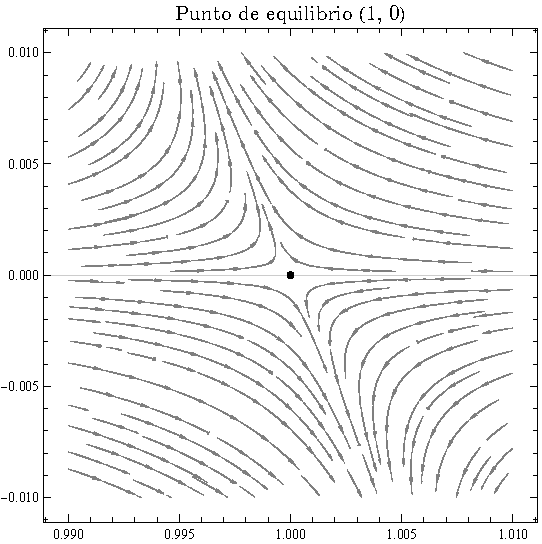
\includegraphics[width=.8\textwidth]{../img/puntoDeEquilibrio(1,0).pdf}
					\caption{\centering Simulación numérica del retrato de fase local cerca de $(1,0)$.}
				\end{figure}
			\end{column}
		\end{columns}
	\end{frame}
	
	\subsection{Desingularización del Origen}
	
	\begin{frame}{Blow-up Polar en $(0,0)$}
		El origen $(0,0)$ es un punto degenerado con $Df(0,0) = \mathbf{0}$. Considerando el campo vectorial $Y_{\eta}(u,v)=f_1(u,v)\dfrac{\partial}{\partial u}+f_2(u,v)\dfrac{\partial}{\partial v}$ donde $\eta=(A,B,Q)$, aplicando la transformación polar $u = r \cos\theta, \; v = r \sin\theta$ y cancelando el factor $r$, el flujo en la frontera $r=0$ está dado por:
		\begin{equation*}
			\bar{Y}_\eta(0,\theta) = A^2 \big[(B-1)\cos\theta - B\sin\theta\big] \cos\theta \sin\theta,
		\end{equation*}
		revelando tres puntos críticos en el primer cuadrante $\theta \in [0, \pi/2]$:
		\begin{enumerate}
			\item $\theta_1 = 0$ (eje $u$)
			\item $\theta_2 = \frac{\pi}{2}$ (eje $v$)
			\item $\theta_3 = \arctan\left(\frac{B-1}{B}\right)$ (existente en el primer cuadrante $\iff B > 1$).
		\end{enumerate}
		
		\begin{block}{Matriz Jacobiana en la Frontera del Cilindro $r=0$}
			\begin{equation*}
				D\bar{Y}_\eta(0,\theta) = \begin{bmatrix}
					A^2 \cos^3\theta + A^2 B (\cos\theta\sin^2\theta - \sin^3\theta) & 0 \\[4pt]
					A^2 \cos^3\theta \sin\theta & b_{22}(\theta)
				\end{bmatrix},
			\end{equation*}
			con $b_{22}(\theta) = A^2 B (\sin^3\theta + \cos^3\theta - 2\sin^2\theta\cos\theta - 2\sin\theta\cos^2\theta) + A^2 (2\cos\theta\sin^2\theta - \cos^3\theta)$.
		\end{block}
	\end{frame}
	
	\begin{frame}{Estructura Sectorial del Origen}
		Evaluando los equilibrios $(0,\theta_j), \; j=1,2,3;$ en la matriz jacobiana $D\bar{Y_{\eta}}(0,\theta)$ obtenemos:
		\begin{itemize}
			\item \textbf{En $\theta_1 = 0$:} $\lambda_r = A^2 > 0$, $\lambda_\theta = A^2(B-1)$. Silla si $B < 1$, Fuente si $B > 1$, Silla-nodo si $B = 1$.
			\item \textbf{En $\theta_2 = \frac{\pi}{2}$:} $\lambda_r = -A^2 B < 0$, $\lambda_\theta = A^2 B > 0$. Punto Silla.
			\item \textbf{En $\theta_3$ (para $B > 1$):} $\lambda_r > 0$, $\lambda_\theta < 0$. Silla radialmente inestable.
		\end{itemize}
		
		\begin{columns}
			\begin{column}{0.45\textwidth}
				\begin{exampleblock}{Índice de Poincaré y Naturaleza Local}
					El origen $(0,0)$ posee índice de Poincaré $I = \frac{e-h}{2} + 1 = 0$ y se comporta localmente como una \textbf{Silla--Nodo} independientemente de los parámetros.
					\begin{itemize}
						\item \textbf{Si $B \le 1$:} Un único sector hiperbólico en el primer cuadrante.
						\item \textbf{Si $B > 1$:} Emerge una separatriz con pendiente $\tan\theta_3 = \frac{B-1}{B}$ que divide el flujo en un sector hiperbólico y uno parabólico.
					\end{itemize}
				\end{exampleblock}
			\end{column}
			
			\begin{column}{0.5\textwidth}
				\centering
				\begin{figure}
					\begin{subfigure}{.45\textwidth}
						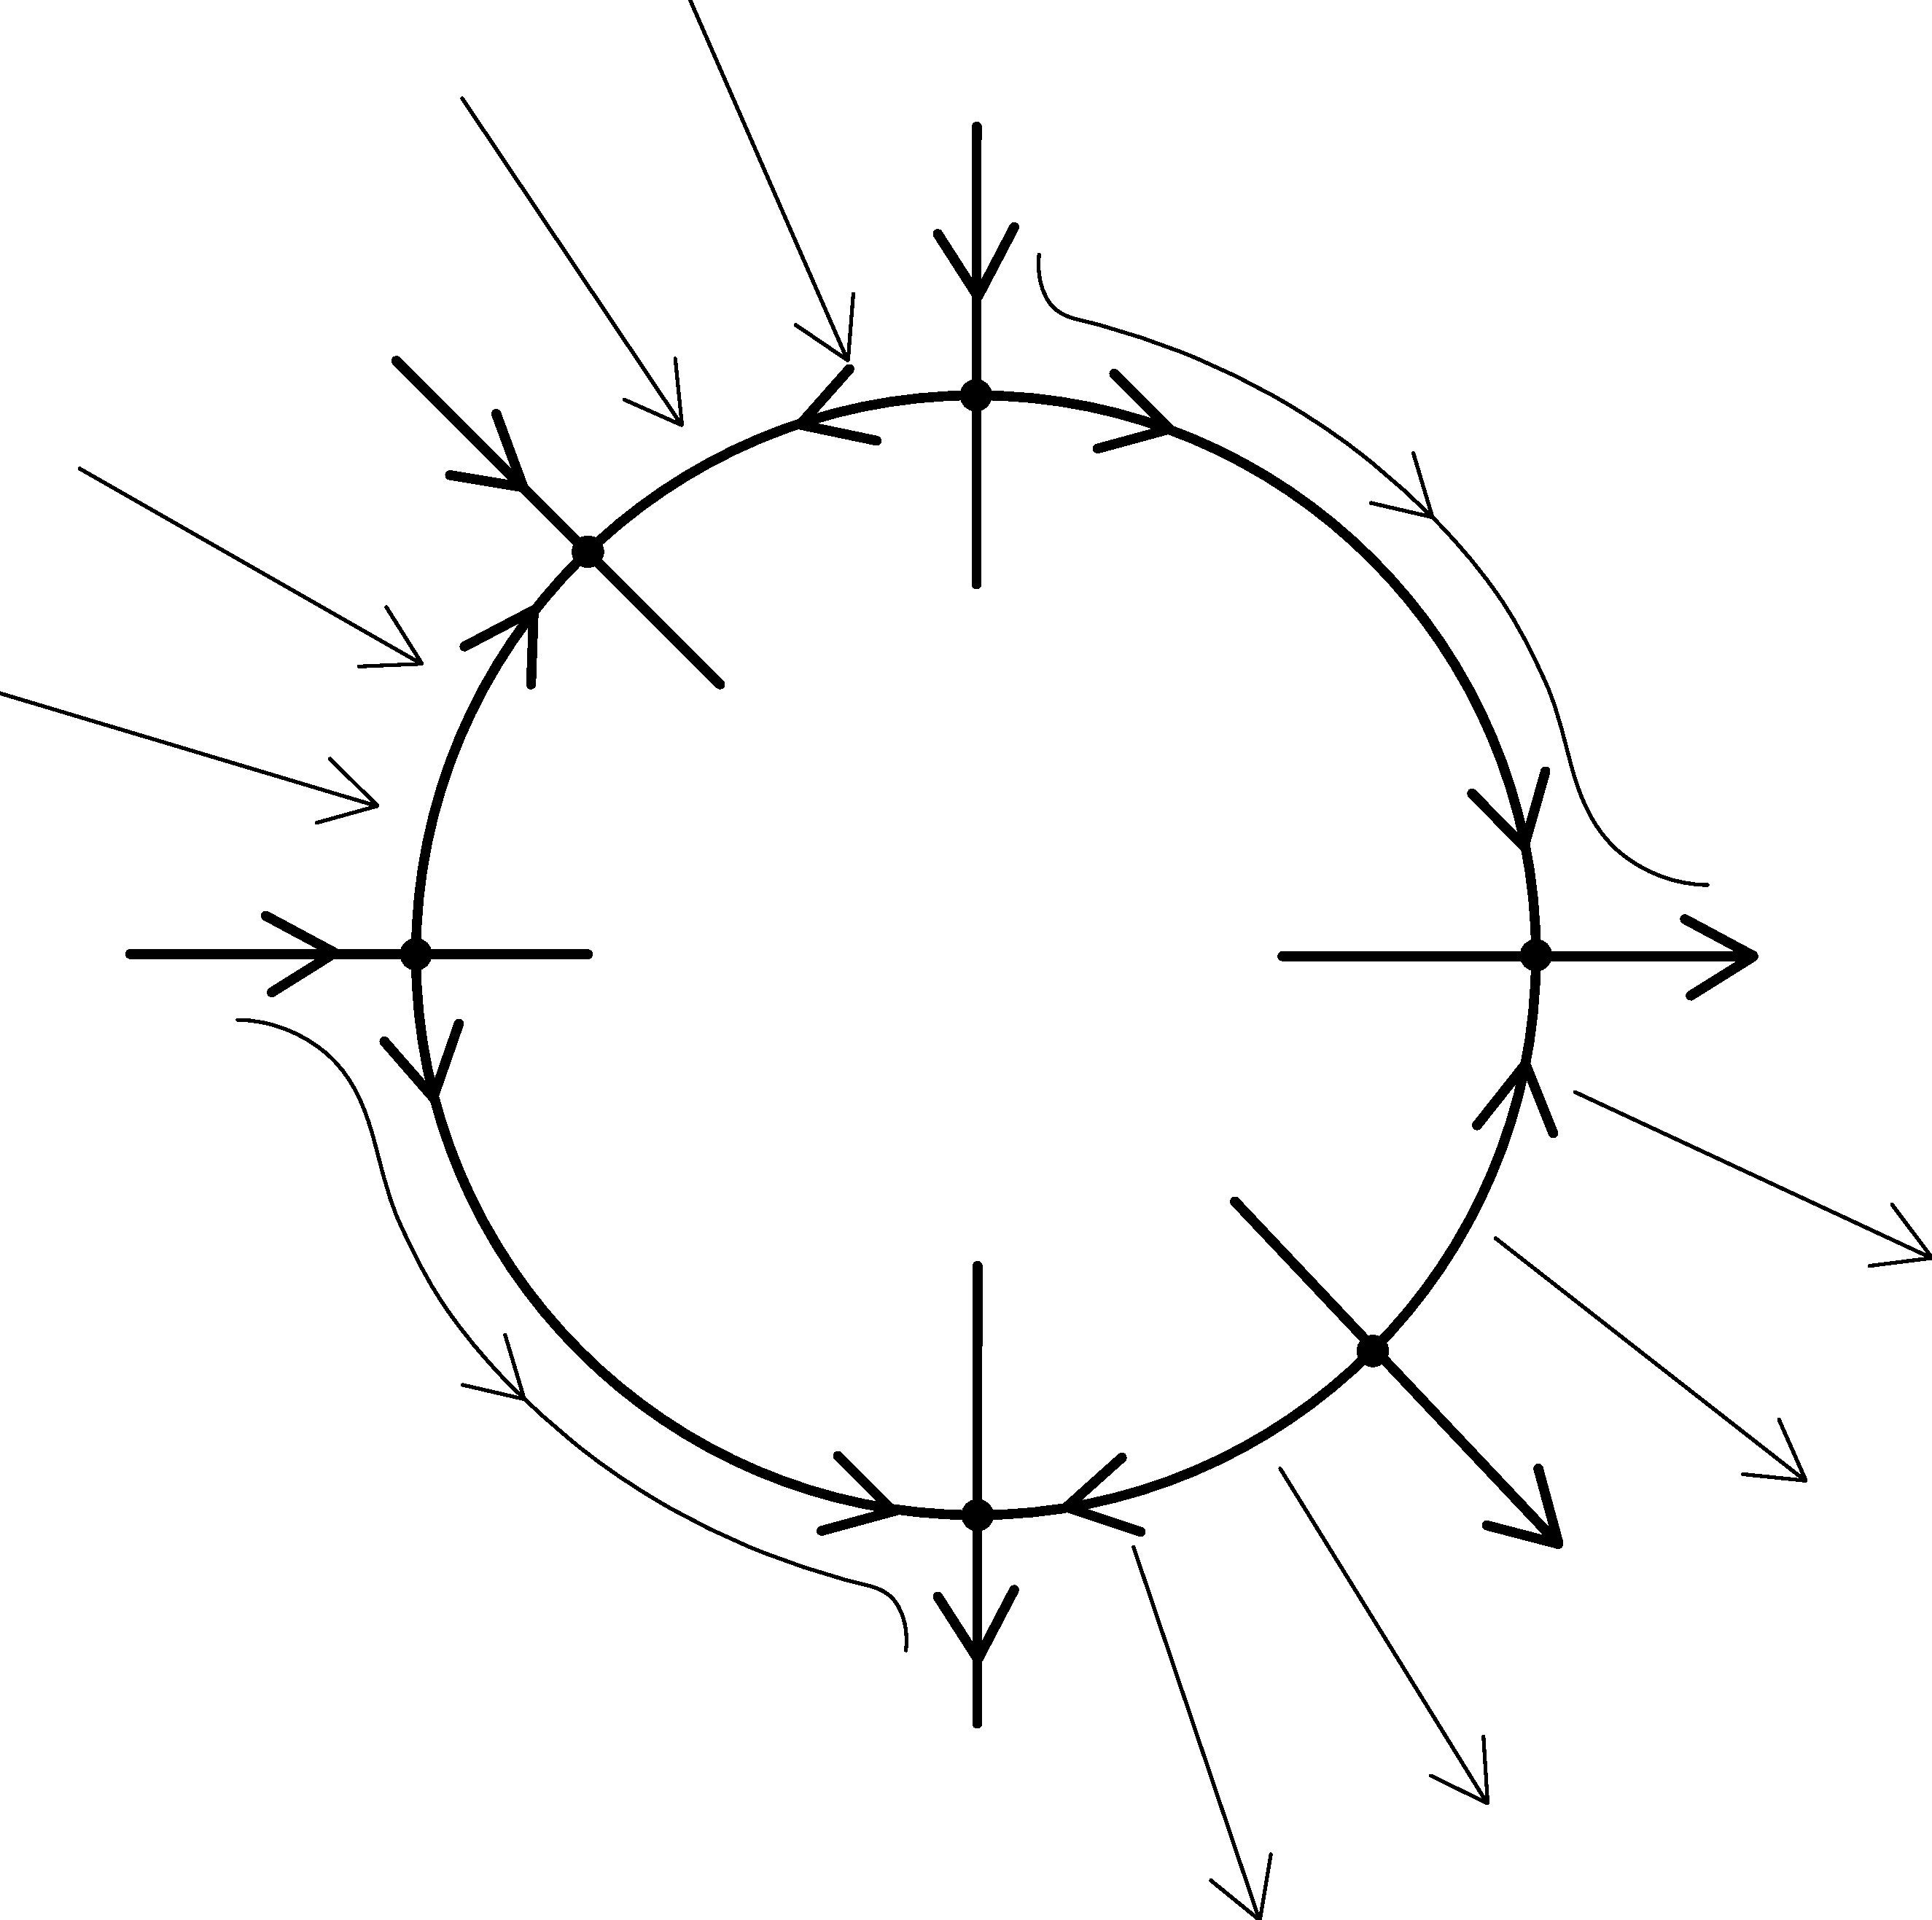
\includegraphics[width=\textwidth]{../img/blowingUpPolar(Bmen1).pdf}
						\caption{$B < 1$.}
					\end{subfigure}
					\begin{subfigure}{.51\textwidth}
						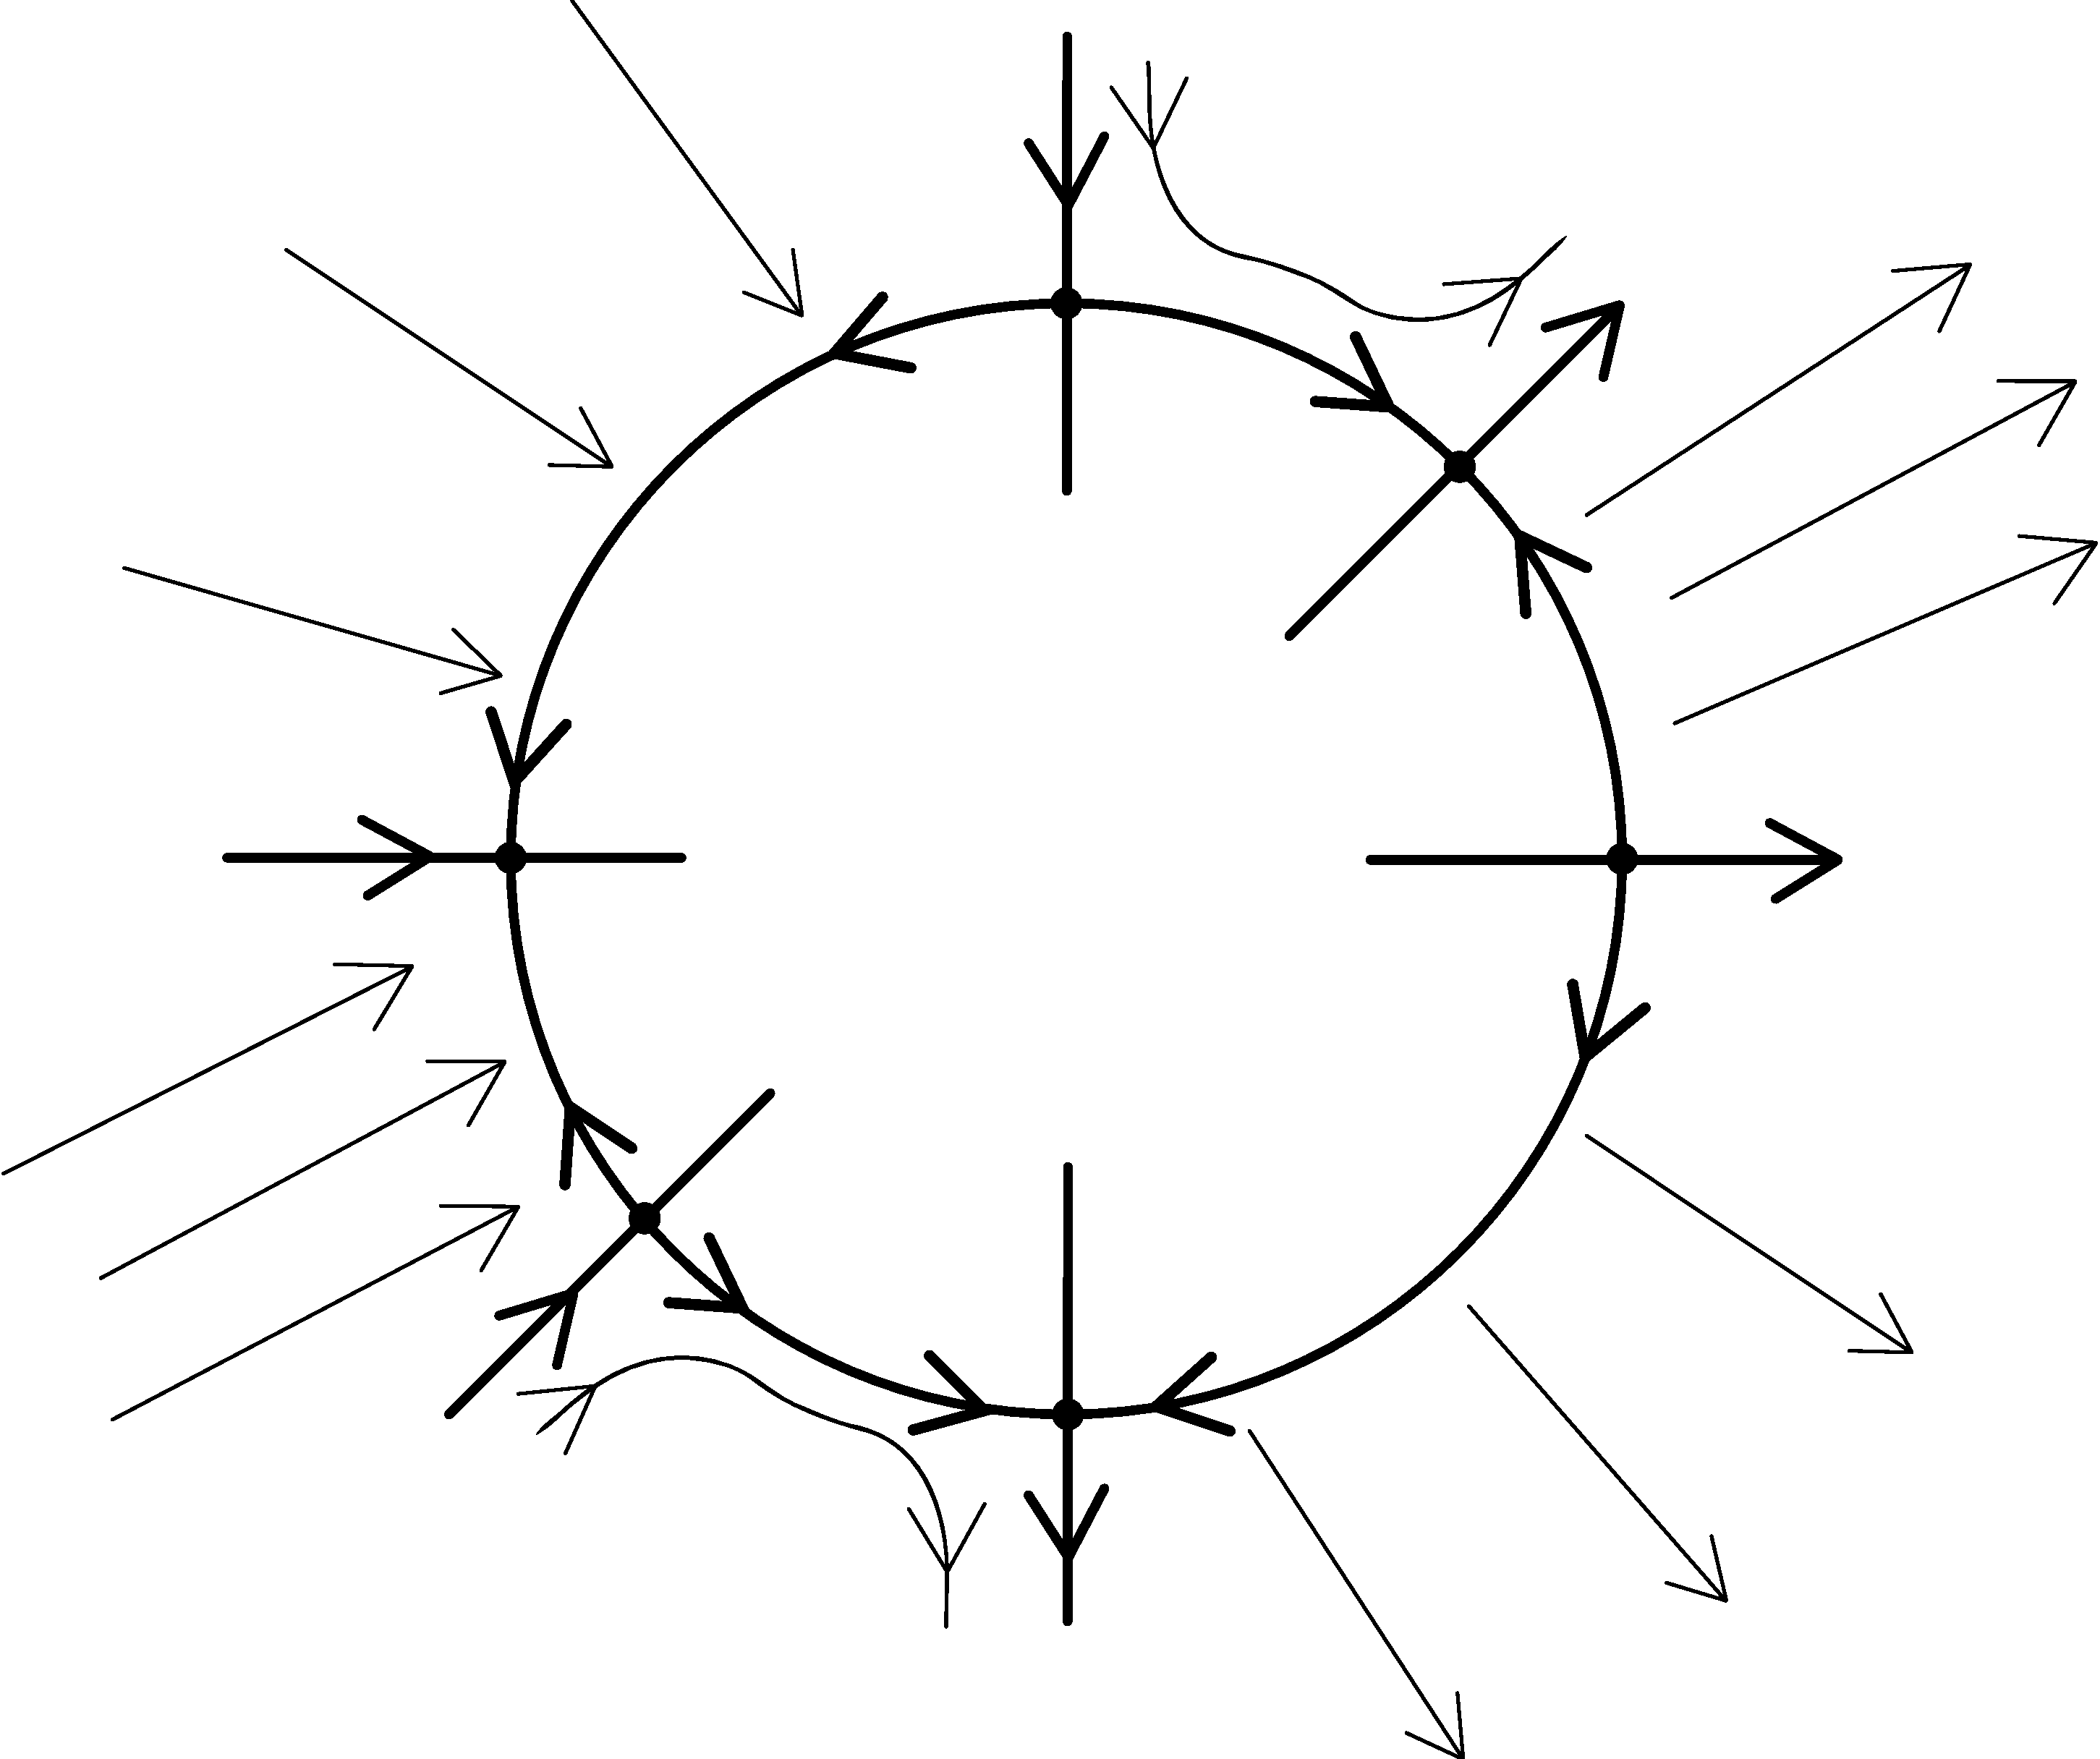
\includegraphics[width=\textwidth]{../img/blowingUpPolar(Bmay1).pdf}
						\caption{$B > 1$.}
					\end{subfigure}
					\caption{Blow-up en el origen del sistema adimensional para diferentes valores de $B$.}
				\end{figure}
			\end{column}
		\end{columns}
	\end{frame}
	
	\begin{frame}{Simulación Numérica del Retrato de Fase cerca de $(0,0)$}
		\centering
		\begin{figure}
			\centering
			\begin{subfigure}[t]{0.4\textwidth}
				\centering
				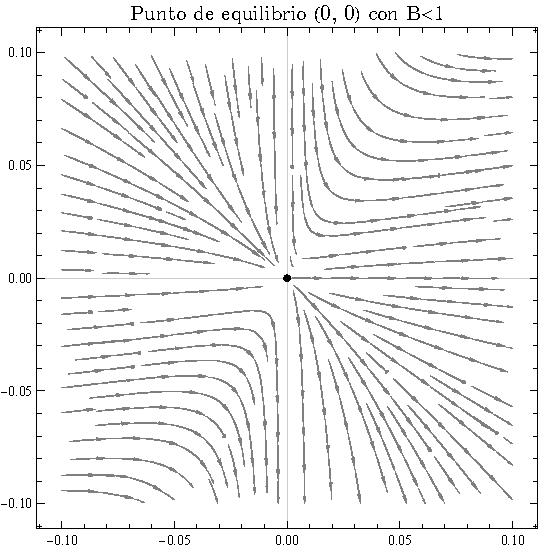
\includegraphics[width=\textwidth]{../img/puntoDeEquilibrio(0,0)conBmenor1Version2.pdf}
				\caption{$B \le 1$: Único sector hiperbólico en el primer cuadrante.}
				\label{fig:origen_b_menor}
			\end{subfigure}
			\begin{subfigure}[t]{0.4\textwidth}
				\centering
				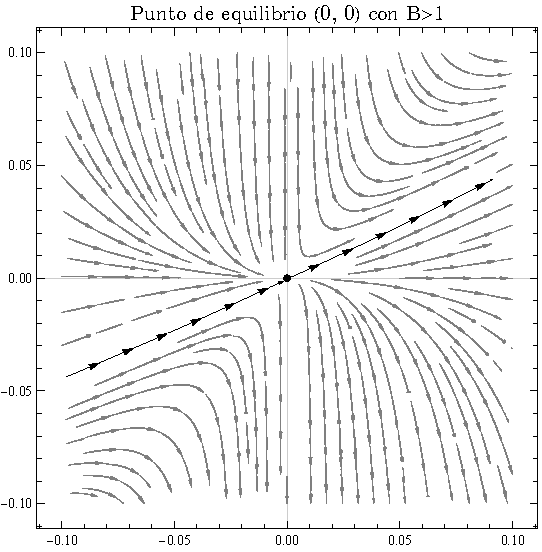
\includegraphics[width=\textwidth]{../img/puntoDeEquilibrio(0,0)conBmayor1Version2.pdf}
				\caption{$B > 1$: Aparición de separatriz en el primer cuadrante.}
				\label{fig:origen_b_mayor}
			\end{subfigure}
			\caption{Validación numérica del retrato de fase local en el origen degenerado.}
		\end{figure}
	\end{frame}
	
	\subsection{Estabilidad del Punto de Coexistencia (H,H)}
	
	\begin{frame}{Estabilidad del Punto de Coexistencia $(H,H)$}
		Sustituyendo $Q = \dfrac{(1-H)(A^2+H^2)}{H^2}$ en la matriz jacobiana $Df(H,H)$:
		\begin{equation*}
			Df(H,H) = \begin{bmatrix}
				-H\big(H^2(2H-1)+A^2\big) & -H(1-H)(A^2+H^2) \\[4pt]
				B H (A^2+H^2) & -B H (A^2+H^2)
			\end{bmatrix},
		\end{equation*}
		con
		\begin{align*}
			\operatorname{tr}(Df(H,H)) &= -H \Big( B(A^2+H^2) + H^2(2H-1) + A^2 \Big), \\[4pt]
			\det(Df(H,H)) &= B H^2 (A^2+H^2) \Big( H^3 + A^2(2-H) \Big) > 0.
		\end{align*}
		
		\begin{block}{Valor Crítico de Hopf ($B_c$)}
			La traza se anula en $B_c = \dfrac{H^2(1-2H) - A^2}{A^2+H^2} < 1$ (requiriendo $H < \frac{1}{2}$ y $A^2 < H^2(1-2H)$):
			\begin{itemize}
				\item \textbf{Si $B < B_c$:} $(H,H)$ es un \textbf{Repulsor} (foco/nodo inestable) y existe al menos un ciclo límite estable en $\Gamma$.
				\item \textbf{Si $B > B_c$:} $(H,H)$ es un \textbf{Atractor} (foco/nodo estable).
			\end{itemize}
		\end{block}
	\end{frame}
	
	\begin{frame}{Primer Coeficiente de Lyapunov ($l_1$) y Bifurcación de Hopf}
		Para $B = B_c$, $(H,H)$ es un \textbf{centro lineal}. El cálculo explícito del primer coeficiente de Lyapunov determina la estabilidad en este caso:
		\begin{equation*}
			l_1 = \dfrac{2A^2(1-H) \left\{ \big[4 - 3H(3-H)\big] A^4 - 4H^3 A^2 - (3-H)H^5 \right\}}{(A^2+H^2) \left\{ \big[H^3 + A^2(2-H)\big]\big[H^2(1-2H)-A^2\big] \right\}^{3/2}}.
		\end{equation*}
		El coeficiente $l_1$ se anula en el valor crítico $A_c = \sqrt{\dfrac{2H^3 + H^2(1-H)\sqrt{3H(4-H)}}{4 - 3H(3-H)}}$ para $H \in \left(0, \frac{3-\sqrt{6}}{3}\right)$:
		
		\begin{itemize}
			\item \textbf{Si $A < A_c \implies l_1 < 0$:} \textbf{Bifurcación de Hopf Supercrítica}. $(H,H)$ es un foco débil inestable rodeado por un ciclo límite estable.
			\item \textbf{Si $A > A_c \implies l_1 > 0$:} \textbf{Bifurcación de Hopf Subcrítica}. $(H,H)$ es un foco débil estable rodeado por un ciclo límite inestable y este a su vez por un ciclo límite estable.
		\end{itemize}
	\end{frame}
	
	\begin{frame}{Bifurcación de Bautin (Hopf Generalizada)}	
		\begin{columns}[c]
			\begin{column}{0.52\textwidth}
				Para $B = B_c$ y $A = A_c$, el primer coeficiente se anula ($l_1 = 0$).
				\begin{alertblock}{Segundo Coeficiente de Lyapunov ($l_2$) y Bautin}
					El cálculo numérico del segundo coeficiente de Lyapunov arroja $l_2 < 0$ para todo $H \in \left(0, \frac{3-\sqrt{6}}{3}\right)$.
					\begin{itemize}
						\item Ocurre una \textbf{Bifurcación de Bautin} (Hopf generalizada) de codimensión 2.
						\item El punto $(H,H)$ es un \textbf{foco débil estable de segundo orden}.
						\item Coexisten dos ciclos límites concéntricos: un ciclo límite inestable interior y un ciclo límite estable exterior.
					\end{itemize}
				\end{alertblock}
			\end{column}
			
			\begin{column}{0.45\textwidth}
				\centering
				\begin{figure}
					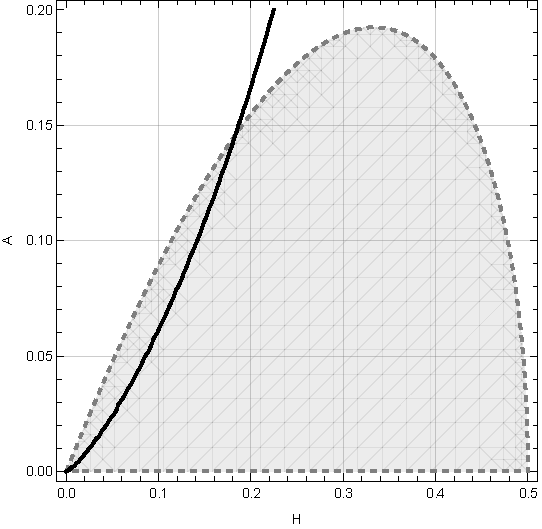
\includegraphics[width=.9\textwidth]{../img/CurvaLyapunovAH.pdf}
					\caption{\centering Curva $l_1 = 0$ y la región dada por las restricciones  $H < \dfrac{1}{2}, \; A^2 < H^2(1 - 2H)$.}
				\end{figure}
			\end{column}
		\end{columns}
	\end{frame}
	
	\begin{frame}{Simulación Numérica: Bifurcación de Hopf}
		Estudio comparativo del comportamiento dinámico en torno al punto de coexistencia $(H,H)$ según el signo del primer coeficiente de Lyapunov $l_1$:
		\begin{columns}[T]
			\begin{column}{0.48\textwidth}
				\begin{block}{Caso Supercrítico ($l_1 < 0$)}
					\centering
					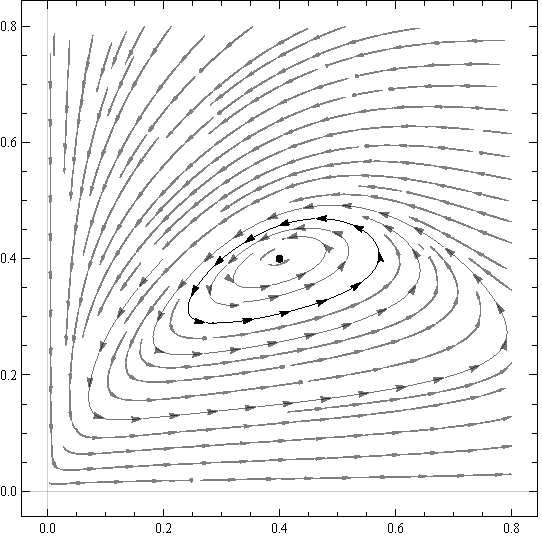
\includegraphics[width=0.55\textwidth]{../img/HopfSuperCentrolineal.pdf}
					
					\vspace{0.1cm}
					\raggedright
					{\scriptsize
						\textbf{Parámetros:} $A = 0.05$, $H = 0.4$, $B_c = 0.1815$, $Q = 0.6094$.\\[2pt]
						\textbf{Dinámica:} $(H,H)$ es un foco débil \textbf{inestable}, el cual repele las trayectorias hacia un único \textbf{ciclo límite estable}.
					}
				\end{block}
			\end{column}
			\begin{column}{0.48\textwidth}
				\begin{exampleblock}{Caso Subcrítico ($l_1 > 0$)}
					\centering
					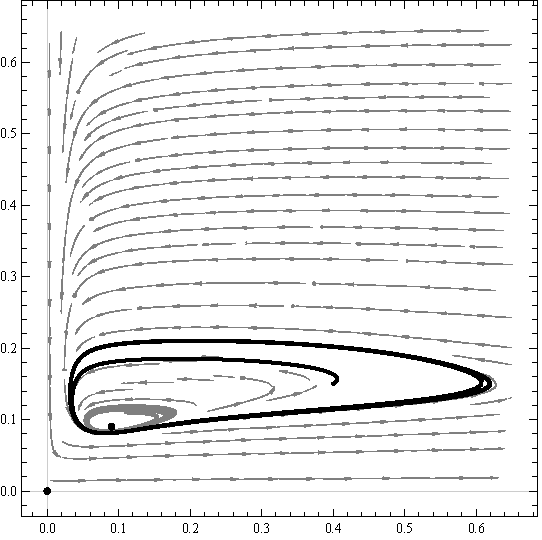
\includegraphics[width=0.55\textwidth]{../img/HopfSubCentrolinealVersion2.pdf}
					
					\vspace{0.1cm}
					\raggedright
					{\scriptsize
						\textbf{Parámetros:} $A = 0.078$, $H = 0.4$, $B_c = 0.0643$, $Q = 1.594$.\\[2pt]
						\textbf{Dinámica:} $(H,H)$ es un foco débil \textbf{estable}, rodeado por un \textbf{C.L. inestable} interior y un \textbf{C.L. estable} exterior.
					}
				\end{exampleblock}
			\end{column}
		\end{columns}
	\end{frame}
	
	% =============================================================================
	% SECCIÓN 4: CONCLUSIONES
	% =============================================================================
	\section{Conclusiones}
	
	\begin{frame}{Conclusiones Principales}
		\begin{enumerate}
			\item \textbf{Invariancia Positiva:} Se demostró rigurosamente que el cuadrado unitario $\Gamma = \{ (u,v) \in \mathbb{R}^2 \mid 0 \le u \le 1, \; 0 \le v \le 1 \}$ es un conjunto positivamente invariante, garantizando la acotación y consistencia biológica de las soluciones.
			\item \textbf{Punto Silla Universal $(1,0)$:} El estado libre de depredadores es un punto silla hiperbólico para cualquier combinación de parámetros.
			\item \textbf{Singularidad en el Origen $(0,0)$:} La desingularización mediante blow-up polar clasificó el origen como un punto \textbf{Silla--Nodo} ($I=0$) para cualquier combinación de parámetros. Para $B > 1$, se encontró que el primer cuadrante contiene una separatriz inestable respecto al origen, cuya dirección está determinada por $\tan\theta_3 = \frac{B-1}{B}$.
			\item \textbf{Bifurcaciones de Coexistencia $(H,H)$:} Se establecieron las condiciones analíticas exactas para la bifurcación de Hopf ($B = B_c$) y la bifurcación de Bautin ($B = B_c, \; A = A_c$), demostrando la aparición de oscilaciones persistentes y ciclos límites concéntricos múltiples.
		\end{enumerate}
	\end{frame}
	
	% =============================================================================
	% SECCIÓN 5: REFERENCIAS
	% =============================================================================
	\section{Referencias Principales}
	
	\begin{frame}{Referencias Principales}
		\begin{thebibliography}{99}
			\bibitem{dumortier}
			Dumortier, F., Llibre, J., y Artés, J.~C. (2006).
			\newblock \emph{Qualitative Theory of Planar Differential Systems}.
			\newblock Universitext, Springer-Verlag, Berlin Heidelberg.
			
			\bibitem{articulo}
			González-Olivares, E., Tintinago-Ruiz, P.~C., y Rojas-Palma, A. (2015).
			\newblock A Leslie--Gower-type predator--prey model with sigmoid functional response.
			\newblock \emph{International Journal of Computer Mathematics}, 92(9), 1895--1909.
			
			\bibitem{kuznetsov}
			Kuznetsov, Yu.~A. (2023).
			\newblock \emph{Elements of Applied Bifurcation Theory}.
			\newblock 4th edition, Springer Nature Switzerland AG.
			
			\bibitem{perko}
			Perko, L. (2001).
			\newblock \emph{Differential Equations and Dynamical Systems}.
			\newblock 3rd edition, Springer-Verlag, New York.
		\end{thebibliography}
	\end{frame}
	
	% -----------------------------------------------------------------------------
	% SLIDE FINAL
	% -----------------------------------------------------------------------------
	\begin{frame}
		\centering
		\vspace{1cm}
		{\Huge \textbf{\color{BlueAccent} ¡Muchas Gracias!}} \\[1.5cm]
		{\large ¿Preguntas o Comentarios?}
	\end{frame}
	
\end{document}